\documentclass[a4paper,12pt]{article}
\usepackage[T2A]{fontenc}
\usepackage[utf8x]{inputenc}
\usepackage[english,russian]{babel}
\usepackage{amssymb,amsfonts,amsmath,mathtext}
\usepackage[unicode]{hyperref}
\usepackage{listings}
\usepackage{graphicx}
\usepackage{float}
\graphicspath{{images/}}
\newcommand{\anonsection}[1]{\section*{#1}\addcontentsline{toc}{section}{#1}}

\begin{document}

% Титульный лист

\begin{titlepage}
\newpage

\begin{center}

\textit{Министерство науки и высшего образования Российской Федерации \\ 
Федеральное государственное бюджетное образовательное \\
учреждение высшего образования \\
«Московский государственный технический университет \\
имени Н.Э. Баумана (национальный исследовательский университет)» \\
(МГТУ им. Н.Э. Баумана) \\}
\hrulefill
\end{center}

\vspace{2em}

\begin{flushleft}
ФАКУЛЬТЕТ <<Информатика и системы управления>> \\
\vspace{0.5em}
КАФЕДРА <<Программное обеспечение ЭВМ и информационные технологии>>
\end{flushleft}


\vspace{8em}

\begin{center}
\LARGE Лабораторная работа №8 \\
\end{center}

\vspace{1.5em}

\begin{center}
\textsc{Поиск в словаре}
\end{center}

\vspace{6em}

\begin{center}
Головнев Н.В.

\vspace{4em}

ИУ7-54Б
\end{center}

\vspace{\fill}

\begin{center}
Москва 2019
\end{center}

\end{titlepage}

\tableofcontents

% Введение

\newpage
\anonsection{ВВЕДЕНИЕ}
Алгоритмы поиска в слова - алгоритмы, определяющие наличие найденного в тексте слова в некой коллекции данных, которая называется словарем.

\newpage
\anonsection{ПОСТАНОВКА ЗАДАЧИ}
Необходимо реализовать алгоритм поиска слов в словаре. Эффективность алгоритма должна составлять не более $\log_2N$, где N - размер сегмента словаря (кол-во слов), в котором производится поиск.

\newpage
\section{АНАЛИТИЧЕСКАЯ ЧАСТЬ}
\subsection{Описание алгоритма}


\newpage
\subsection{Вывод}
Аналитически 

% Конструкторская часть

\newpage
\section{КОНСТРУКТОРСКАЯ ЧАСТЬ}

\subsection{Разработка алгоритмов}
На вход у всех алгоритмов передаются в качестве параметров:
\begin{enumerate}
\item Словарь (Дерево) (указатель или ссылка);
\item Строка, которая ищется в словаре;
\item Длина этой строки;
\item Переменная в которую будет записан результат (указатель или ссылка);
\end{enumerate}
Возвращаемое значение: код ошибки (0 в случае успеха, иначе отрицательное значение). \\
Побочные эффекты: изменяется значение переменной результата.

\newpage
\subsection{Схемы алгоритмов}
%Ниже представлены схемы алгоритмов сортировок (сортировка пузырьком, сортировка минимум/максимум, шейкерная сортировка).

\newpage
\subsection{Вывод}
На основе аналитических данных были разработаны требования к разрабатываемым алгоритмам.


\newpage
\section{ТЕХНОЛОГИЧЕСКАЯ ЧАСТЬ}
\subsection{Требования к программному обеспечению}

Программа должна работать на операционной системе Arch Linux. 
Программа должна запускаться из консоли (или терминала) следующей командой:\\
\textit{./app.exe dictionary.txt text.txt} \\
\textit(app.exe) - само приложение. \textit{dictionary.txt} - файл со словами, которые хранит в себе словарь. На каждой строке должно располагаться одно слово без разделительных знаков. \text{text.txt} - файл с текстом, в котором ищутся слова, отсутствующие в словаре.
На выход программа должна печатать все слова, не найденные в этом словаре.

\newpage
\subsection{Средства реализации}
Для реализации данных алгоритмов был выбран язык программирования С, компилятор gcc и некоторые функции из библиотеки glibc (memcpy, malloc и тд...). \\

\newpage
\subsection{Листинг кода}
Ниже приведены реализации алгоритмов на С.\\
\lstdefinestyle{customc}{
  belowcaptionskip=1\baselineskip,
  breaklines=true,
  frame=L,
  xleftmargin=\parindent,
  language=C,
  showstringspaces=false,
  basicstyle=\footnotesize\ttfamily
}

\newpage
\subsection{Вывод}
Используя язык программирования C, в ходе практической работы был спроектирован и написан алгоритм поиска в словаре.

\newpage
\section{ЭКСПЕРИМЕНТАЛЬНАЯ ЧАСТЬ}
\subsection{Характеристики аппаратного и программного обеспечения}
% Часть которую никогда нельзя менять
Тестирование приложения проводилось на машине со следующими характеристиками:\\
\begin{itemize}
\item Процессор Intel® Core™ i7-7700HQ;
\item Оперативная память 16 ГБ;
\item Операционная система - Arch Linux с рабочим окружением Gnome 3.
\end{itemize}

\newpage
\subsection{Примеры работы}
На Рис. \ref{images:example}, предсавленном ниже, демонстрируется работа приложения. Запуск приложения осуществляется из эмулятора терминала в Arch Linux. Во время работы приложение запрашивает у пользователя параметры массива и выводит результаты сортировки на экран.
\begin{figure}[h]
\center{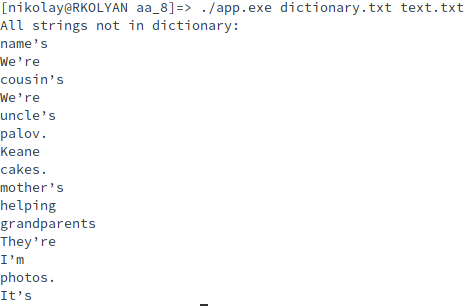
\includegraphics[scale=0.5]{example.png}}
\caption{Пример работы приложения}
\label{images:example}
\end{figure}

\newpage
\subsection{Оценка затрачиваемой памяти}
Размер памяти (в байтах) $M$, выделенной под словарь можно вычислить по формуле:\\
\begin{equation}
M =  \sum_{i = 0}^{\vert V \vert} T_i + P * \vert V \vert
\end{equation}
где:\\
\begin{equation}
T_i = \left\{
\begin{array}{ll}
\vert V \vert * \alpha + \sum_{j = 0}^N T_{ij} + \beta + P\text{,} & \text{if } T_i \text{ exists} \\
0\text{,} & \text{if } T_i \text{ not exists} \\
\end{array}
\right.
\end{equation}
$V$ - заданный алфавит, \\
$\alpha$ - размер символа в байтах, \\
$\beta$ - размер переменной счетчика(если тип integer - 4 байт),\\
$N$ - кол-во дочерних узлов дерева словаря (значение счетчика), \\
$P$ - память, выделяемая под указатели.

\newpage
\subsection{Вывод}
В результате исследования оценки времени выполнения можно сделать вывод, что сортировка пузырьком имеет самые худшие временные показатели. Сортировка методом поиска минимума и максимума самая быстрая и не зависит от расположения элементов. Для того, чтобы не наблюдалось случая, как представлено на графике[\ref{images:graphics1}], достаточно сделать вначале проверку на сортированость.

\newpage
\anonsection{ЗАКЛЮЧЕНИЕ}
Поиск в словаре в основном нужен для проверки орфографии в редакторах текста. Также, он ускоряет написание программ в интегрированных средствах разработки путем автоподставления слов (переменных, функций и тд).

\newpage
\anonsection{СПИСОК ИСТОЧНИКОВ}
\begin{itemize}
\item \label{site:wikipedia}https://ru.wikipedia.org/wiki/
\item \label{site:habr}https://habr.com/ru/post/422085/
\end{itemize}

\end{document}
